% Copyright (c)  2005-2010 EDF-EADS-PHIMECA.
% Permission is granted to copy, distribute and/or modify this document
% under the terms of the GNU Free Documentation License, Version 1.2
% or any later version published by the Free Software Foundation;
% with no Invariant Sections, no Front-Cover Texts, and no Back-Cover
% Texts.  A copy of the license is included in the section entitled "GNU
% Free Documentation License".
\renewcommand{\nomfichier}{docref_C311_TransIso}
\renewcommand{\titrefiche}{Isoprobabilistic transformation preliminary to FORM-SORM methods}

\Header

\MathematicalDescription{
  \underline{\textbf{Goal}} \vspace{2mm}

  The isoprobabilistic transformation is used in the following context : $\vect{X}$ is the input random vector, $F_i$ the cumulative density functions of its components and $C$ its copula.\\

  Let us denote by $\vect{d}$ a deterministic vector, $g(\vect{X}\,,\,\vect{d})$ the limit state function of the model, $\cd_f = \{\vect{X} \in \Rset^n \, / \, g(\vect{X}\,,\,\vect{d}) \le 0\}$ the event considered here and {g(\vect{X}\,,\,\vect{d}) = 0} its boundary.\\

  One way to evaluate the probability content $P_f$ of the event $\cd_f$:
  \begin{equation}\label{PfXIsoProb}
    P_f = \mathbb{P}[g(\vect{X}\,,\,\vect{d})\leq 0]=   \int_{\cd_f} \pdf\, d\vect{x}
  \end{equation}
  is to introduce an isoprobabilistic transformation $T$ which is a diffeomorphism from $\supp(\vect{X})$ into $\mathbb{R}^n$, such that the distribution of the random vector $\vect{U}=T(\vect{X})$ has the following properties : $\vect{U}$ and $\mat{R}\,\vect{U}$ have the same distribution for all rotations $\mat{R}\in\mathcal{SO}_n(\mathbb{R})$. \\

  Such transformations exist and the most widely used are :
  \begin{itemize}
  \item the Generalized Nataf transformation (refer to \otref{docref_C311_TransIso_Generalized Nataf}{Generalized Nataf}),
  \item the Rosenblatt transformation (refer to \otref{docref_C311_TransIso_Rosenblatt}{Rosenblatt}).
  \end{itemize}

  \vspace{2mm}

  \underline{\textbf{Principle}} \vspace{2mm}


  If we suppose that the numerical model $g$ has suitable properties of differentiability, the evaluation of the probability (\ref{PfXIsoProb}) can be transformed in the evaluation of the probability:

  \begin{equation}
    \label{StandardSpace}
    P_f = \mathbb{P}[G(\vect{U}\,,\,\vect{d})\leq 0] = \int_{\mathbb{R}^n} \boldsymbol{1}_{G(\vect{u}\,,\,\vect{d}) \leq 0}\,f_{\vect{U}}(\vect{u})\,d\vect{u}
  \end{equation}
  where $T$ is a $C^1$-diffeomorphism called an \emph{isoprobabilistic transformation}, $f_{\vect{U}}$ the probability density function of $\vect{U}=T(\vect{X})$ and $G=f\circ T^{-1}$.\\
  The vector $\vect{U}$ is said to be in the \emph{standard space}, whereas $\vect{X}$ is in the \emph{physical space}.\\

  The interest of such a transformation is the rotational invariance of the distributions in the standard space : the random vector $\vect{U}$ has a spherical distribution, which means that the density function $f_{\vect{U}}$ is a function of $\|\vect{u}\|$. Thus, without loss of generality, it is possible to map the general failure domain $\mathcal{D}$ to a domain $\mathcal{D}'$ for which the design point ${\vect{u}^{*}}'$ (the point of the event boundary at minimal distance from the center of the standard space) is supported by the last axis (see Figure (\ref{Invariance}).



  % \begin{figure}[Hhtbp]
  \begin{center}
    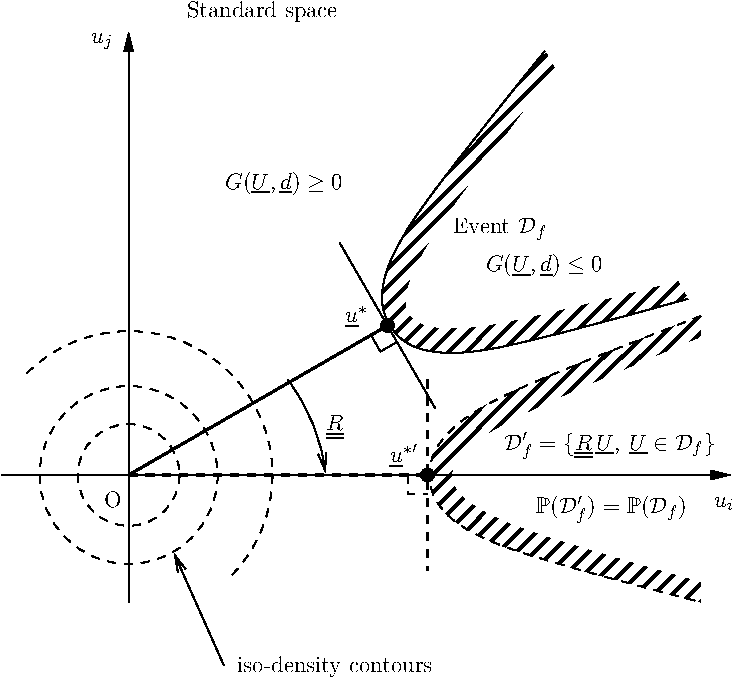
\includegraphics{FigureRotationFinal.pdf}
  \end{center}
  \label{Invariance}
  % \caption{\label{Invariance} Rotational invariance after the application of the iso-probabilistic transformation Nataf, Generalized Nataf or Rosenblatt. }
  % \label{Rotation}
  % \end{figure}

  The following transformations verify that property, under some specific conditions on the dependence structure of the random vector $\vect{X}$ :
  \begin{itemize}
  \item the Nataf transformation (see [A. Nataf]) : $\vect{X}$ must have a normal copula,
  \item the Generalized Nataf transformation (see [R. Lebrun, A. Dutfoy, 2008, b]) : $\vect{X}$ must have an elliptical copula,
  \item the Rosenblatt transformation (see [M. Rosenblatt]) : there is no condition on the copula of $\vect{X}$ .
  \end{itemize}

  Open TURNS uses automatically the Generalized Nataf transformation when the copula is elliptical and the Rosenblatt transformation for any other case.
}
{
  --}

\Methodology{
  Within the global methodology, the isoprobabilistic transformation is used in the First and Second Order Reliability Method to evaluate the probability content of the event $\cd_f$ (refer to \otref{docref_C311_Form}{FORM} and \otref{docref_C311_Sorm}{SORM}).
}
{
  According to the isoprobabilistic transformation used, the standard space differs ([R. Lebrun, A. Dutfoy, 2008, b]) : in the standard space of the Generalized Nataf transformation, distributions are spherical, with zero mean, unit variance and unit correlation matrix. The type of the spherical distribution is the type of the elliptical copula of the initial random vector $\vect{X}$. In the standard space of the Rosenblatt transformation, distributions are normal distributions with zero mean, unit variance and independent components (which is equivalent, in that normal case, to a unit correlation matrix).\\


  The reference [R. Lebrun, A. Dutfoy, 2008, c] makes a comparison between both isoprobabilistic transformations : Generalized Nataf and Rosenblatt. The conclusions are the following ones : In the case where the copula of the random vector $\vect{X}$ is normal, the canonical Rosenblatt transformation (it means when the conditionning order follows the natural order of the components) and the Nataf transformation are identical; if the conditionning order is not the canonical one, both transformations only differ by an orthogonal transformation.\\
  In the case where the copula of the random vector $\vect{X}$ is elliptical without being normal, both transformations differ and both standard spaces can not be compared.\\



  Let's note some usefull references:
  \begin{itemize}
  \item A. Der Kiureghian, P.L. Liu, 1986,"Structural Reliability Under Incomplete Probabilistic Information", Journal of Engineering Mechanics, vol 112, n�1, pp85-104.
  \item R. Lebrun, A. Dutfoy, 2008, b, "A generalisation of the Nataf transformation to distributions with elliptical copula", Probabilistic Engineering Mechanics 24 (2009), pp. 172-178, doi:10.1016/j.probengmech.2008.05.001.
  \item R. Lebrun, A. Dutfoy, 2008, c, "Do Rosenblatt and Nataf isoprobabilistic transformations really differ?", submitted to Probabilistic Engineering Mechanics in august 2008, under review so far.
  \item A. Nataf, "D�termination des distributions de probabilit�s dont les marges sont donn�es", Comptes Rendus de l'Acad�mie des Sciences, 225, 42-43.
  \item M. Rosenblatt, "Remarks on a Multivariat Transformation", The Annals of Mathematical Statistics, Vol. 23, No 3, pp. 470-472.
  \end{itemize}


}

\Example{
  Refer to \otref{docref_C311_TransIso_Generalized Nataf}{Generalized Nataf} or \otref{docref_C311_TransIso_Rosenblatt}{Rosenblatt} to have some examples of isoprobabilistic transformations.
}
